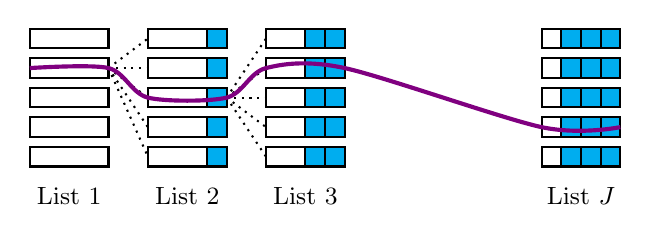
\begin{tikzpicture}
[font=\small, draw=black, line width=0.75pt,
sub0/.style={rectangle, draw, inner sep=0pt, minimum width=10mm, minimum height=2.5mm},
parity/.style={rectangle, draw, fill=cyan, inner sep=0pt, minimum size=2.5mm}]

\foreach \c in {3.00, 2.625, 2.25, 1.875, 1.5} {
  \node[sub0] (subcs1\c) at (-1.00,\c) {};
  \node[sub0] (subcs2\c) at (0.50,\c) {};
  \node[parity] (parity0\c) at (0.875,\c) {};
  \node[sub0] (subcs3\c) at (2.00,\c) {};
  \node[parity] (parity1\c) at (2.125,\c) {};
  \node[parity] (parity2\c) at (2.375,\c) {};
  \node[sub0] (subcsz\c) at (5.50,\c) {};
  \node[parity] (parity3\c) at (5.375,\c) {};
  \node[parity] (parity4\c) at (5.625,\c) {};
  \node[parity] (parity5\c) at (5.875,\c) {};
}

\draw[dotted] (-0.50,2.625) -- (0.00,3.00) {};
\draw[dotted] (-0.50,2.625) -- (0.00,2.625) {};
\draw[dotted] (-0.50,2.625) -- (0.00,2.25) {};
\draw[dotted] (-0.50,2.625) -- (0.00,1.875) {};
\draw[dotted] (-0.50,2.625) -- (0.00,1.50) {};

\draw[dotted] (1.00,2.25) -- (1.50,3.00) {};
\draw[dotted] (1.00,2.25) -- (1.50,2.625) {};
\draw[dotted] (1.00,2.25) -- (1.50,2.25) {};
\draw[dotted] (1.00,2.25) -- (1.50,1.875) {};
\draw[dotted] (1.00,2.25) -- (1.50,1.50) {};

\node (list1) at (-1.00,1) {List~1};
\node (list2) at (0.50,1) {List~2};
\node (list3) at (2.00,1) {List~3};
\node (list4) at (5.50,1) {List~$J$};

\draw [line width=1.5pt,color=violet] plot[smooth, tension=.5] coordinates {
(-1.50,2.625) (-0.50,2.625)
(0.00,2.25) (1.00,2.25)
(1.50,2.625) (2.50,2.625)
(5.00, 1.875) (6.00, 1.875)};
\end{tikzpicture}
